\documentclass{iopart}

\usepackage{graphicx}
\usepackage[margin=2cm]{geometry}

\begin{document}

\title{Shell Notes}

%\verb+TODO: add pictures+

\section{Overview}
The shell is the protective outer layer of the robot that protects the electronics during gameplay and supports the vision pattern. What usually differentiates shells designed by different teams is material, mounting method, and how much of the robot is covered by the shell. Here we discuss a 3D printed shell that attaches itself by clamping to the underside of the midplate with a compliant mechanism printed into the body of the shell.

%Some shells reach down to the bottom of the bot near the baseplate

%In the past Thunderbots's shells have been 3D printed (PLA or PETG or something) and made from a folded sheet of clear polycarbonate which was then spray-painted black around the edges

\section{Background}
\subsection{Beam deflections}

\section{Terminology}
\begin{itemize}
    \item Shell \\
            The part of the robot that encloses the electronics and protects them from impacts.
    \item Vision Pattern
            The pattern of five circles placed on the top of the robot that are seen by the vision cameras which allows the AI to know positions of the robots.
    \item Leaf
            The spring that is printed into the side of the shell and provides the force that secures the shell onto the robot.
    \item Clamp
    The part that is separate from the shell and connected to it by a dowel that it rotates about. Its function is to transfer the spring force from the leaf into a clamping force on the underside of the midplate.
    \item Nub
    The section of the clamp that extends out and makes contact with the leaf.
\end{itemize}

\section{Radio Considerations}
Since the shell encloses most or all of the robot you have to make sure that the shell does not interfere with our ability to communicate with the robot. This means minimizing the use metals or other materials from the shell and mounting system that could act as a parasitic antenna reducing the power received by the radio module.

Past examples of metal use in the shell on Thunderbots is the 2017 shell which had metal crossbar between two stand-offs which supported the shell and in 2022 we tried an aluminum top plate which held the pieces of paper used for vision between it and the top of the shell. The crossbar was removed because it was suspected to cause radio issues and the metal top plate essentially blocked all communication with the robot.

\section{Geometry Restrictions}
\begin{itemize}
    \item The robot must fit within a cylinder that is 15cm tall and 18cm in diameter.
    \item The rear of the shell must allow the battery cage to be removed without removing the shell. (At the moment the battery cage is in the conceptual stage so there are no hard requirements for this.)
    \item The shell needs to not interfere with any of the electrical components (The cap holders, the faceplate, the overall height of the robot)
\end{itemize}

\section{Goals}
The goal is to create a shell that can be quickly fastened and removed without the use of hand tools or removable parts.

We think the best way to achieve this is to create a shell that can clamp itself onto the side of the midplate where the clamp can be released by hand from the underside.

\section{Design}

\subsection{Clamping mechanism}
The shell is secured to the robot by a clamping mechanism that is mostly printed into the shell itself. The midplate is clamped between a block that is part of the shell and the arm of a second piece that rotates about a dowel attached to the shell. The clamping force is provided by a leaf spring which pushes the second arm closed.

\begin{figure}[h!]
    \centering
    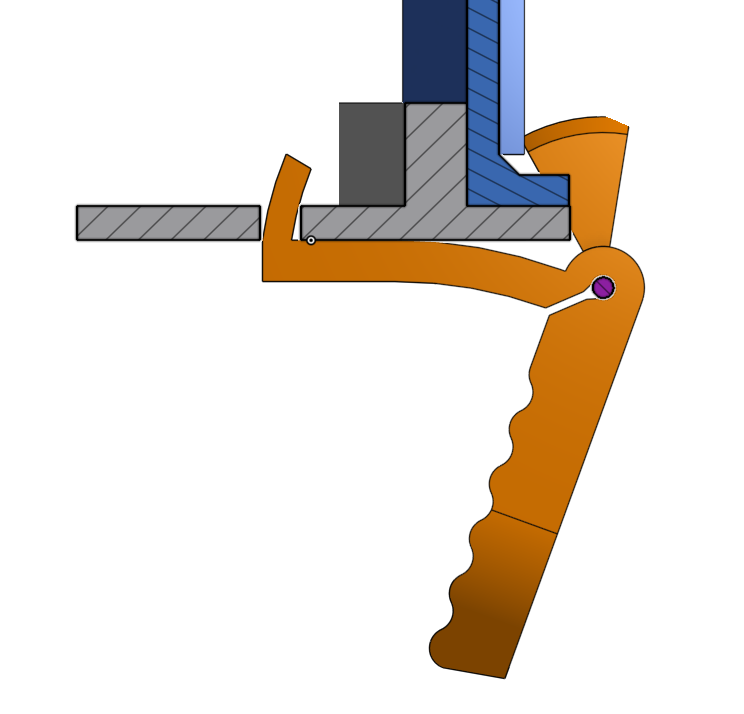
\includegraphics[height=6cm]{graphics/clamp_cross-section.png}
    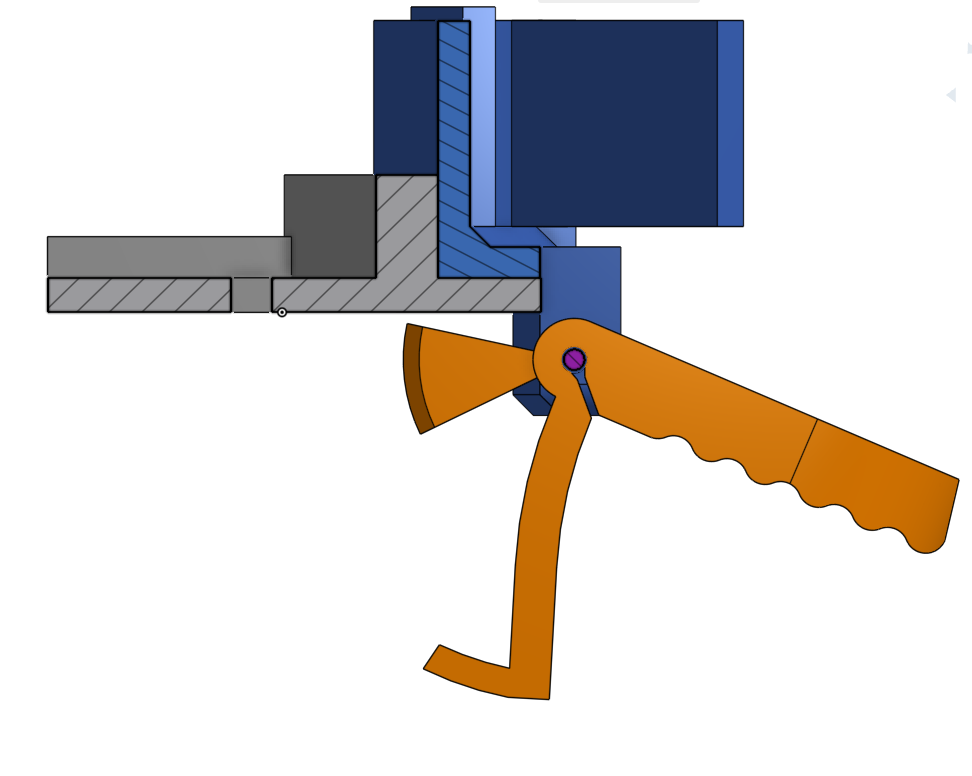
\includegraphics[height=6cm]{graphics/clamp_cross-section2.png}
    \caption{Cross-sectional view of the clamping mechanism, left depicts the clamp in the closed position and right depicts the clamp in the open position.}
\end{figure}

\begin{itemize}
    \item The spring is guided to bend into a circle because this is the shape that evenly distributes the stress
    \item The nub is a wedge because this is the resulting shape of combining many thin rectangular pieces at different angles
    \item Angled portions are cut into the nub so it makes better contact with the spring
    \item There is hook on the clamp arm to better grab onto the midplate and help prevent the shell from rotating.
    \item The clamp flexes open and has a path to fit it over the dowels.
\end{itemize}

\subsection{Print Support}
The top face of the part of the shell that is clamped down onto the midplate is angled up into the shell wall. That is because this section need to be supported during printing the slope makes this section self-supporting. The self-supporting section saves material, saves the effort of removing supports, and makes the shell stronger in that area.

\begin{figure}[h!] 
        \centering       
        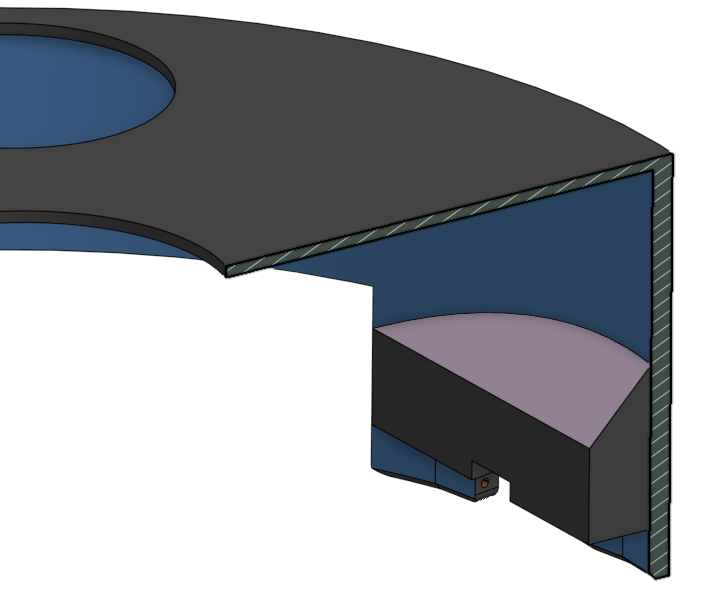
\includegraphics[width=0.6\textwidth]{graphics/shell_print_support.png}
        \caption{View of the clamping section of the shell. The purple face is angled rather than parallel to the top plane to make it self-supporting.}
\end{figure}

\subsection{Spring shape}
\subsection{Battery carriage cutout}

\section{Material Choice}
There seems to be a preference among teams to use PLA filament as a default for 3D printing components likely because it is often the cheapest and easiest filament to print with. We didn't want to use PLA for the shells because compared to other filaments such as ASA and ABS it has low impact resistance and fatigue strength. The exact material properties of ASA and ABS filament depends on the specific blend purchased, and we went with ASA because it was cheaper at the time and has the added benefit of being fire retardant.

\section{Stress and Deflection}
\subsection{Fatigue data}
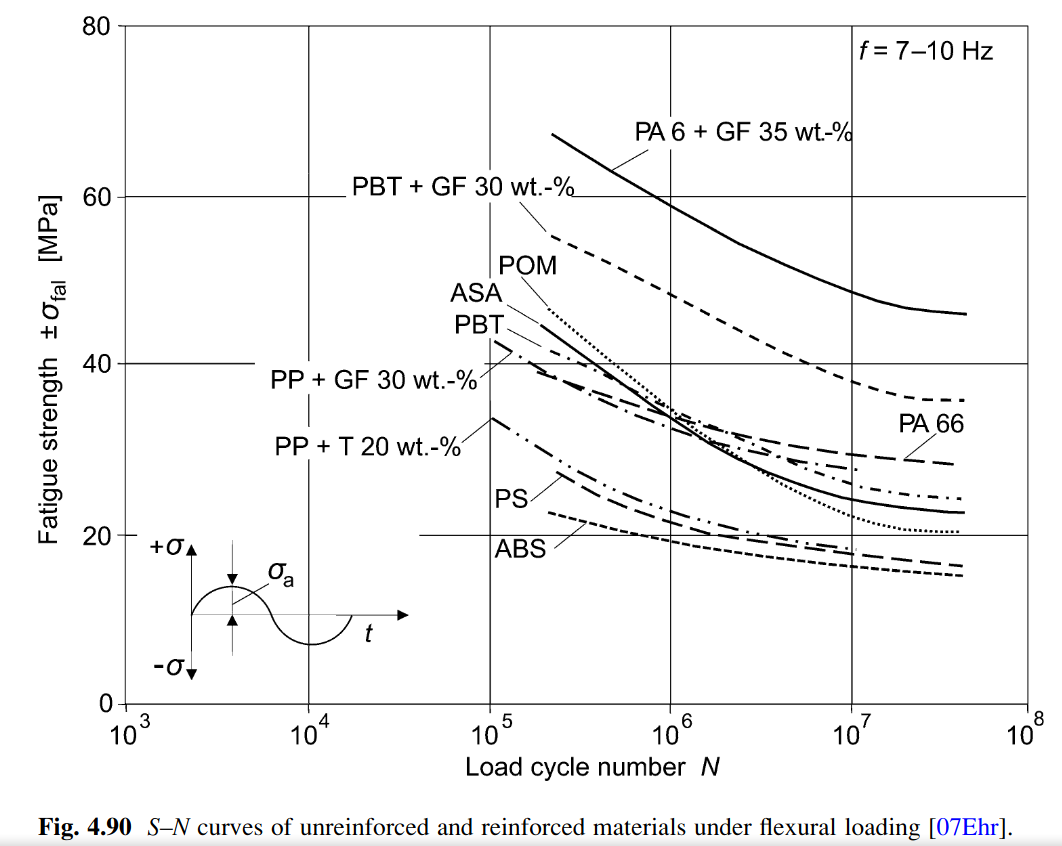
\includegraphics[width=0.8\textwidth]{graphics/alternating_fatigue_strength.png}

Landolt Bornstien cites that the endurance limit $10^7$ cycles for ASA is a stress of 25Mpa. Matter3D states that the flexural modulus of their filament is 2.5GPa
\subsection{Stress vs displacement}
\subsection{Expected force displacement}
\subsection{Impact Failure Energy}
and measured force displacement?

\section{Assembly}
The shell is made of 3D printed components
Say something about adjusting where to put supports to make it easy on yourself
The pins are something you need to buy plus we can simply insert them after printing.
After that you need to insert the clamps and in between the shell and the pins and pull them open around the pin to get them around the pins.

\subsection{3D printing considerations}
The clamps should be printed on their side to maximize the strength of the part by having the flexural stress on the part be along the fibers rather than between the planes.

When printing these parts on their sides the side of the nub that faces the build plate is going to have a worse finish because of the support material because of this I recommend you print these in pairs and alternate whether the right or the left side is up.

You should enable the print thin walls option in Cura to make sure the slicer doesn't try to fill in the gap between the spring and its guide.
\section{Issues}

\section{Iterations}
\subsection{Making the Nub a Wedge}
%\subsection{Pre-Stressing the Leaf}
\subsection{Taking up more midplate space}
\subsection{Qual Bot PLA Version}
\subsection{Getting rid of the dowel path}
\subsection{Creating a guide for how the leaf is allowed to bend}
\subsection{Chamfering the top of the nub}

\section{Past Designs}
\subsection{The Crossbar and rigid columns}
In 2017 on Thunderbots the shell was made from 1/16" pieces of clear polycarbonate that was glued together and painted black. The top of the shell was two thinner pieces that were riveted together, this left a small gap between the two pieces in which small pieces of paper could be placed for the vision colours that were held in place by friction. The shell was secured to the robot via a metal crossbar that went across the top of the robot. The crossbar was threaded to retain two screws that poked up through the top of the shell, two thumb nuts could then be screwed onto the top of the shell securing it between the thumb nuts and the crossbar. The metal crossbar was phased out because it was suspected to cause radio problems. 

Thunderbots had also used some similar designs to this including removing the crossbar by using having columns with a threaded end that poked up through the shell and 3D printing the crossbar out of plastic. 

\begin{figure}[h!]
    \centering
    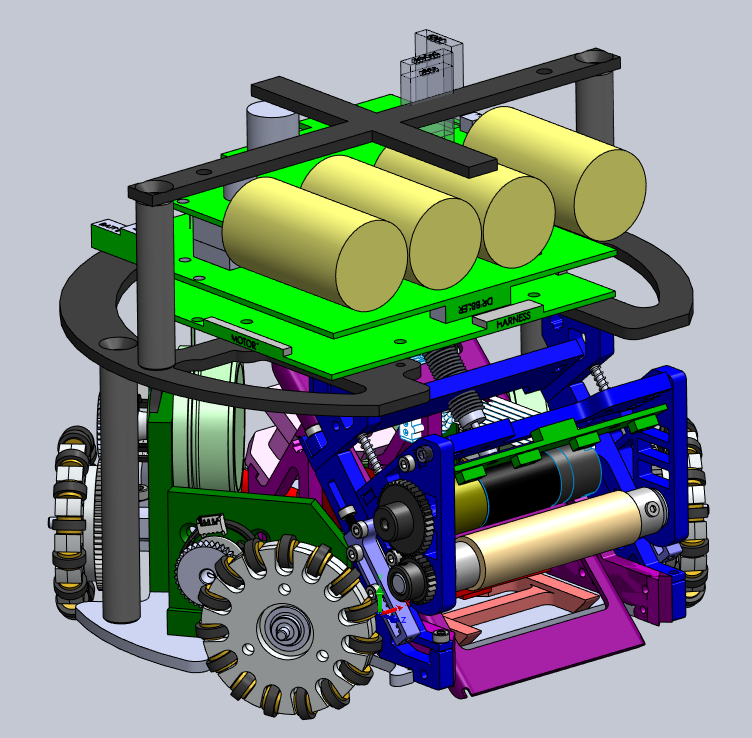
\includegraphics[width=0.5\textwidth]{graphics/crossbar.png}\\
    2017 bot with a crossbar going across the top of the robot to support the shell. The outer holes are for a screw to fasten it to the frame of the robot and the inner pair of holes contained screws for the thumb nuts that secured the shell.
\end{figure}

\subsection{Detent Pin}
An attempt to eliminate the need for a crossbar and the collumns was to have two detent pins on the sides of the midplate that would engage with holes in the side of the shell. The issues with this design were that the shell would sometimes rotate about the line passing through both pins and the shell could also pop off of the pins during gameplay.

\begin{figure}[h!]
    \centering
    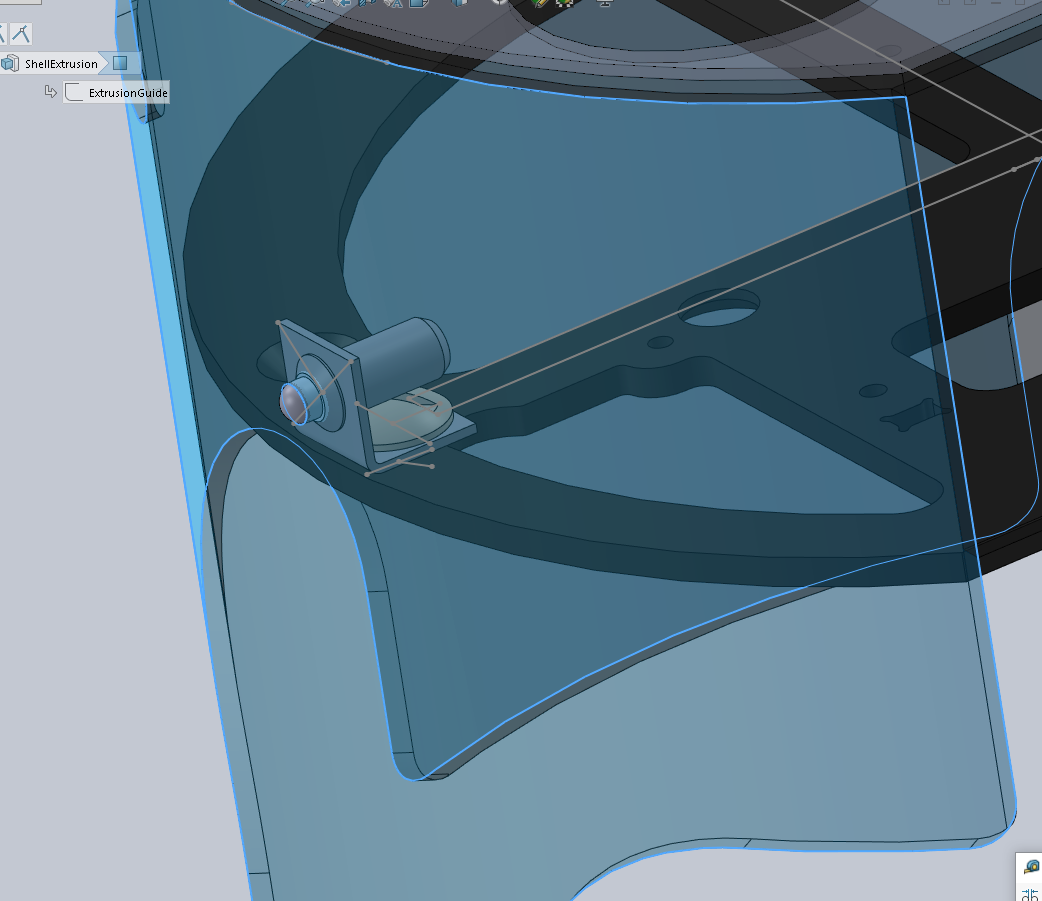
\includegraphics[width=0.5\textwidth]{graphics/detent.png}\\
    Approximate model of the detent pin design, the pin on the tested version didn't extend past the outside of the shell because of the maximum diameter rule.
\end{figure}

\subsubsection{A "flexible" 3D printed shell}

Another attempt to make a shell that was easy to remove and could be attached to the sides of the robot was to make a shell with fingers glued to the inside that could grab onto the sides of the robot. The shell would then be attached and removed by flexing the bottom end of the shell outwards such that it could be pulled over the robot and elastically fasten itself to the midplate. This design was tried at the same time we switched to 3D printing our shells I don't remember what material we tried but it wasn't flexible enough and was prone to breaking along the layers.

\begin{figure}[h!]
    \centering
    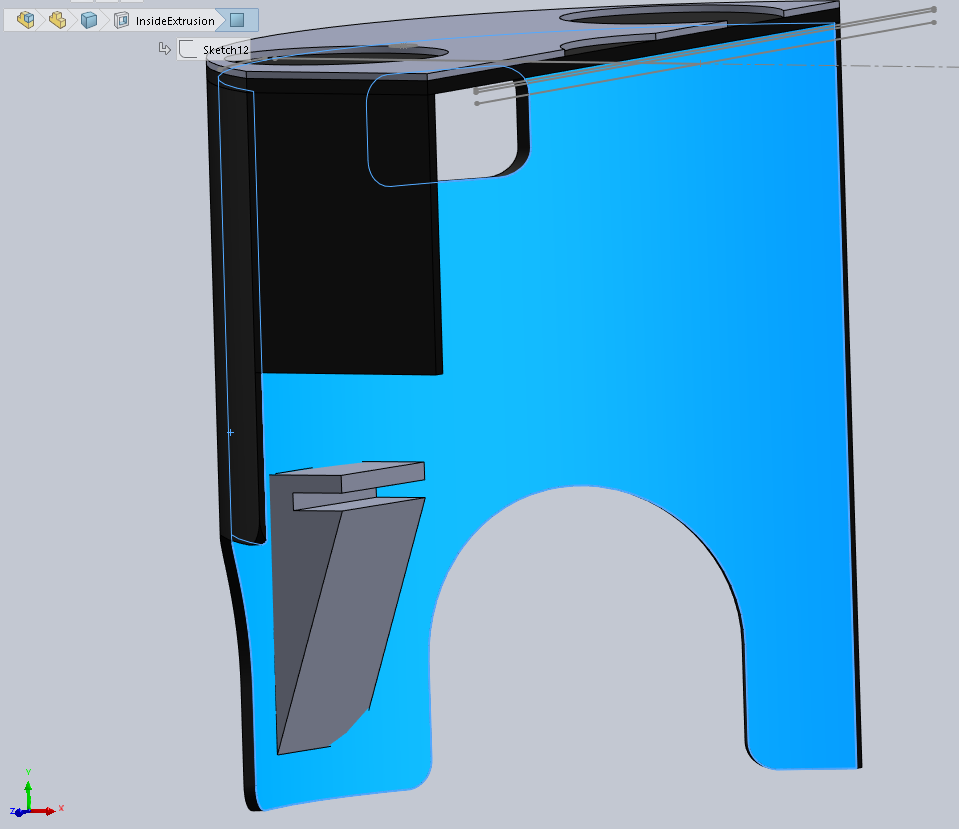
\includegraphics[width=0.5\textwidth]{graphics/flexible_shell.png}\\
    Approximate model of the flexible shell, the wedge attached to the inside of the shell has a cutout to grab onto the midplate.
\end{figure}

\section{Rejected Designs}
\subsection{Clothes Pin Clamping}
The first idea for a shell that fastens itself to shell by clamping onto the underside of the robot was a clothes pin shaped clamp. The idea is a that a tooth would engage into a hole in the underside of the chassis and midplate which would prevent the shell from rotating. Flat sections would extend out from the inside of the shell to prevent the shell from being raised or lowered in this position. To remove the shell you would press a button on the underside of the shell to release the clamp which would allow you to rotate it to a position where there is a cutout section in the midplate which would then allow you to lift the shell straight up to remove it.

\begin{figure}[h!]
    \centering
    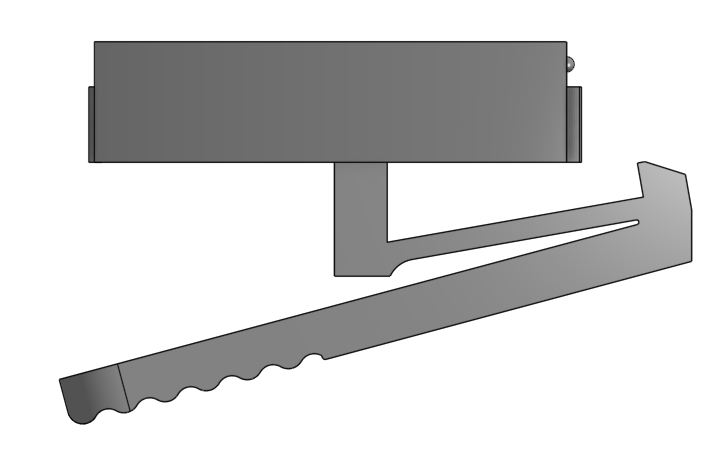
\includegraphics[width=0.5\textwidth]{graphics/clothespin_clamp.png}\\
    Cad model for a prototype version of the clothespin design. The top of the motor mount and the midplate would be pinched between the right side and both would have a hole for the tooth to engage in.
\end{figure}

\begin{figure}[h!]
    \centering
    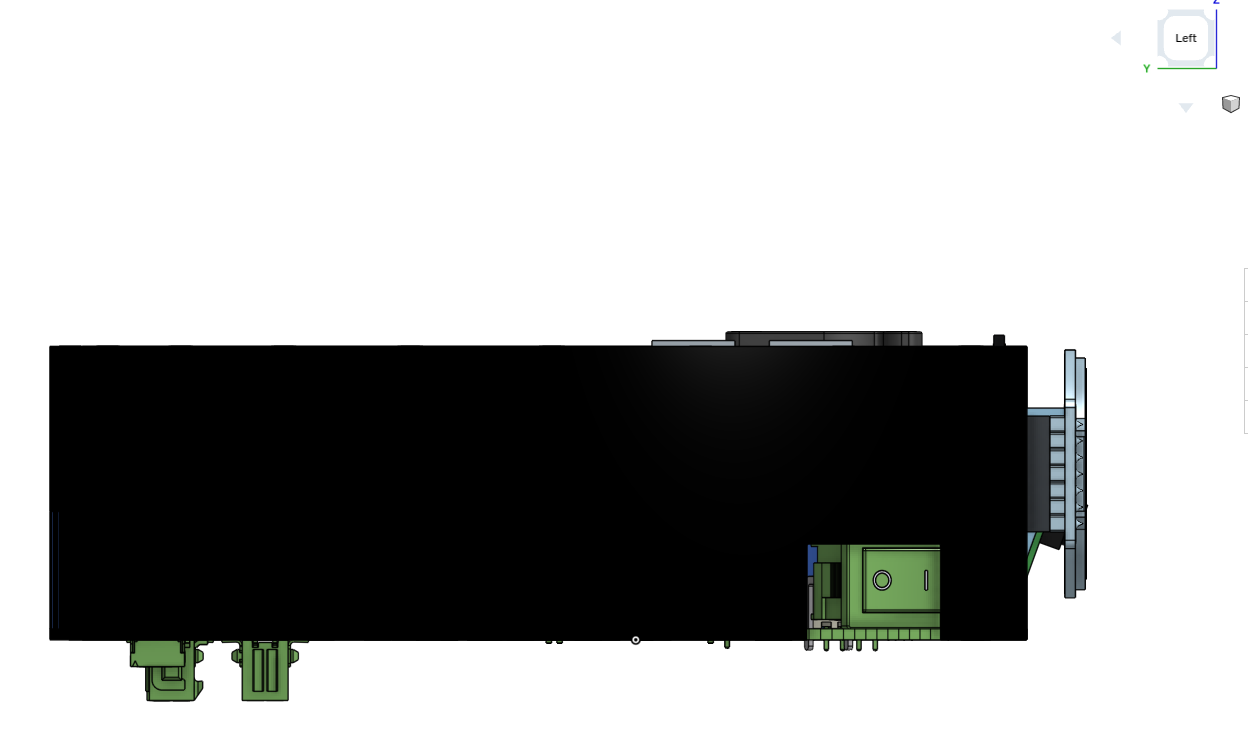
\includegraphics[width=0.3\textwidth]{graphics/clothespin_shell_removal1.png}
    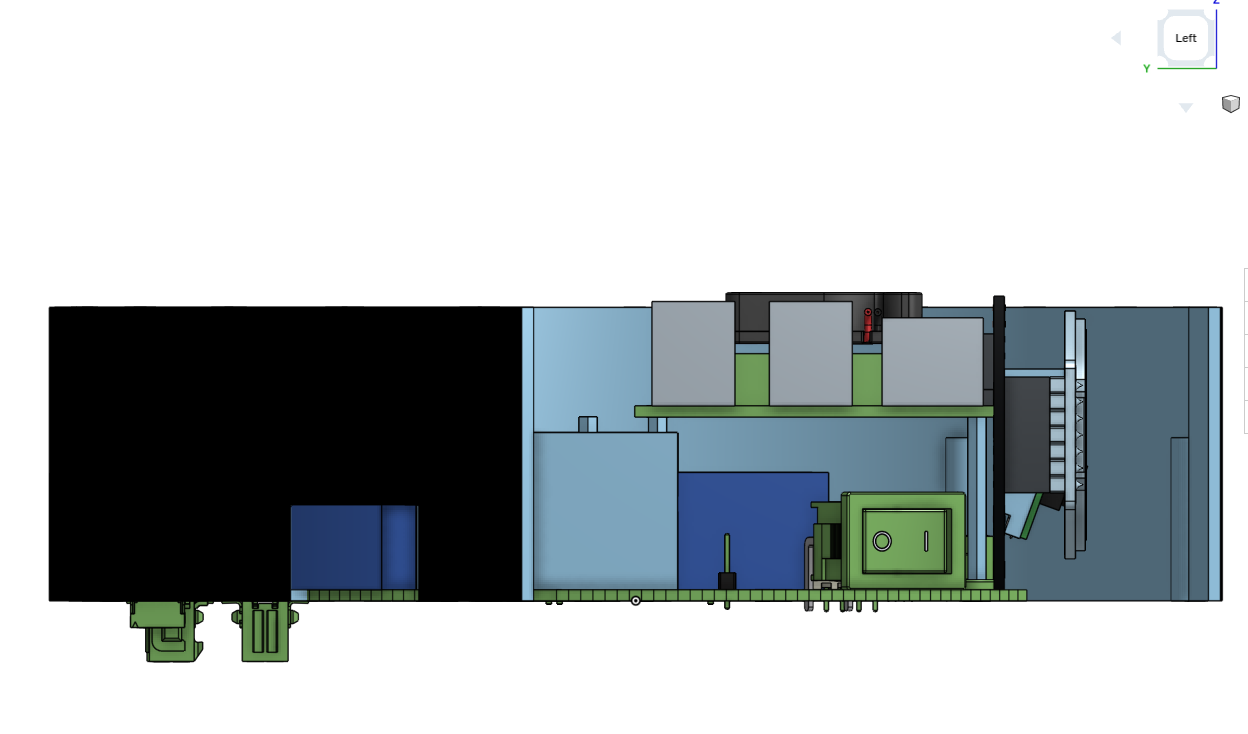
\includegraphics[width=0.3\textwidth]{graphics/clothespin_shell_removal2.png}
    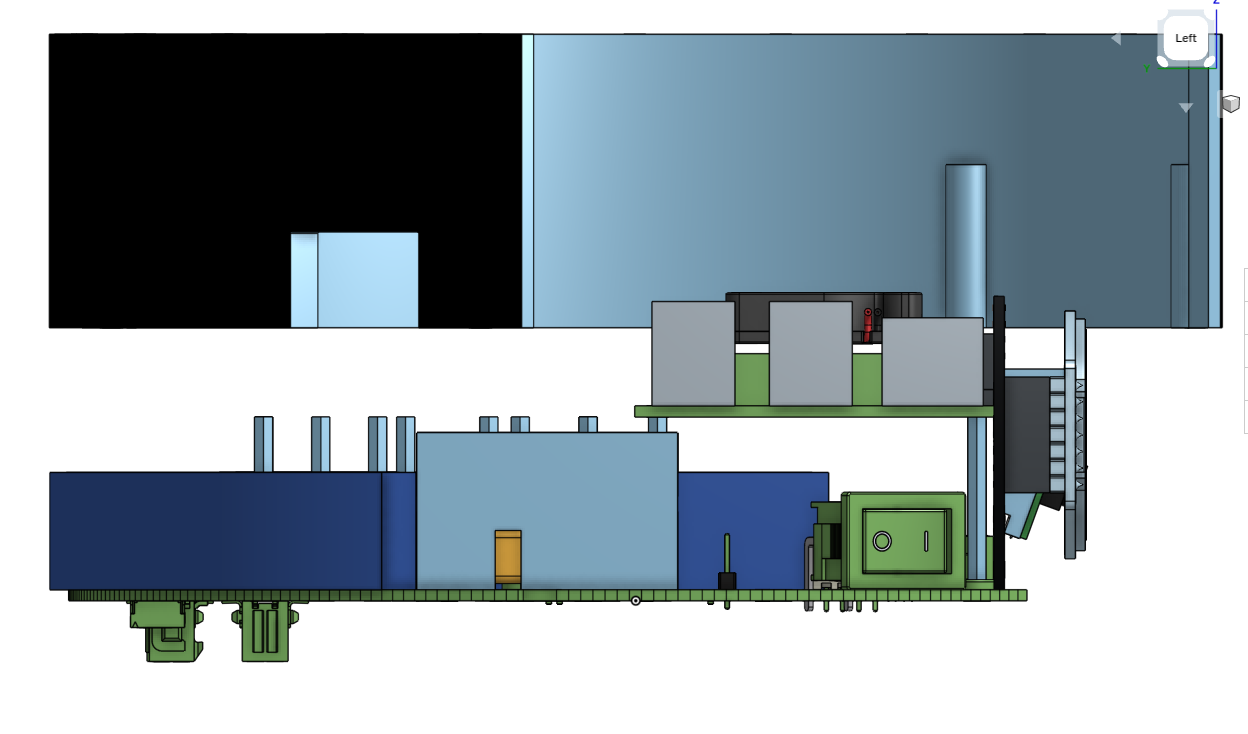
\includegraphics[width=0.3\textwidth]{graphics/clothespin_shell_removal3.png}
    Visualization of the motion that would have been used to remove the shell.
\end{figure}

The main issues with this design were that a lot of space above the midplate had to be cleared out to allow the shell to rotate especially the faceplate and battery cage would have to be made smaller to let the shell rotate around it. There was also not enough space to make this clamp big enough securely hold the shell without yielding. The main space constraints with the clamp we ran into were the wheels the motor mount opposite the one that was being latched onto and cap holders.

\begin{figure}[h!]
    \centering
    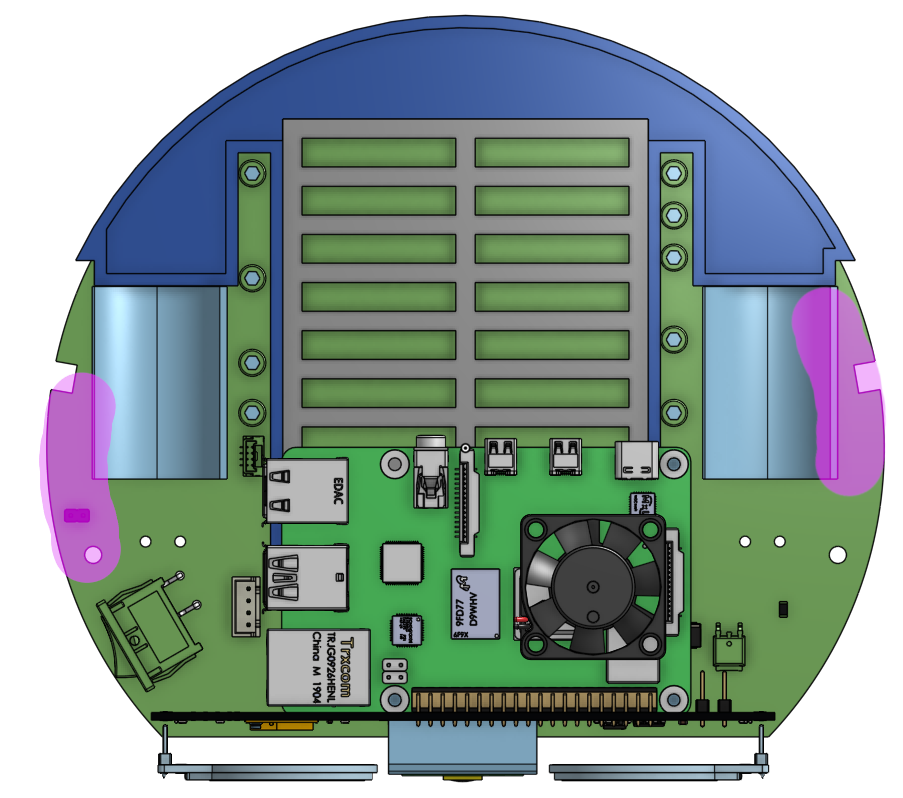
\includegraphics[width=0.6\textwidth]{graphics/clothespin_midplate_clearance.png}\\
    Purple shaded area is a lower bound for the space that would need completely empty for the clothespin design to work.
\end{figure}

This general idea might be feasible with a clamp that isn't a single 3D printed part.

\subsection{Displacement Inverter}

This idea tries to preserve the main idea of the clothes pin design by changing the shape of what engages and disengages the tooth. This idea never got past basic dimensioning as it would face the same interference problems of the previous design and would probably have very similar yielding problems.

\begin{figure}[h!]
    \centering
    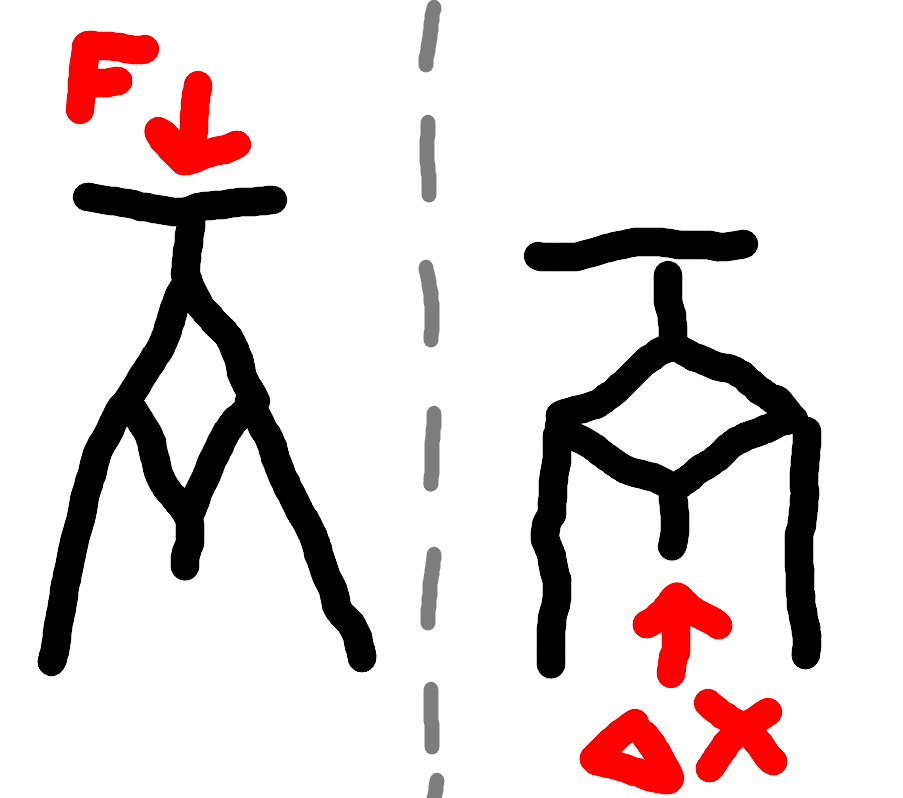
\includegraphics[width=0.5\textwidth]{graphics/displacement_inverter.png}\\
    Basic drawing of a displacement inverter where pressing on one side retracts the opposite end.
\end{figure}

\subsection{Flexible Nub}

The next idea was to change the piece that clamps to underside of the midplate such that it is able to swing out from underneath the midplate allowing the shell to be lifted straight off. The clamp would have a flexible nub that rests against the shell providing resistance that stops it from coming undone during gameplay but if pulled hard enough by the handle would completely flex past the shell allowing it to be removed. The arm that clamps onto the underside of the midplate would also be flexible enough that pushing the handle inwards would allow the nub to be reset latching the shell onto the robot.

\begin{figure}[h!]
    \centering
    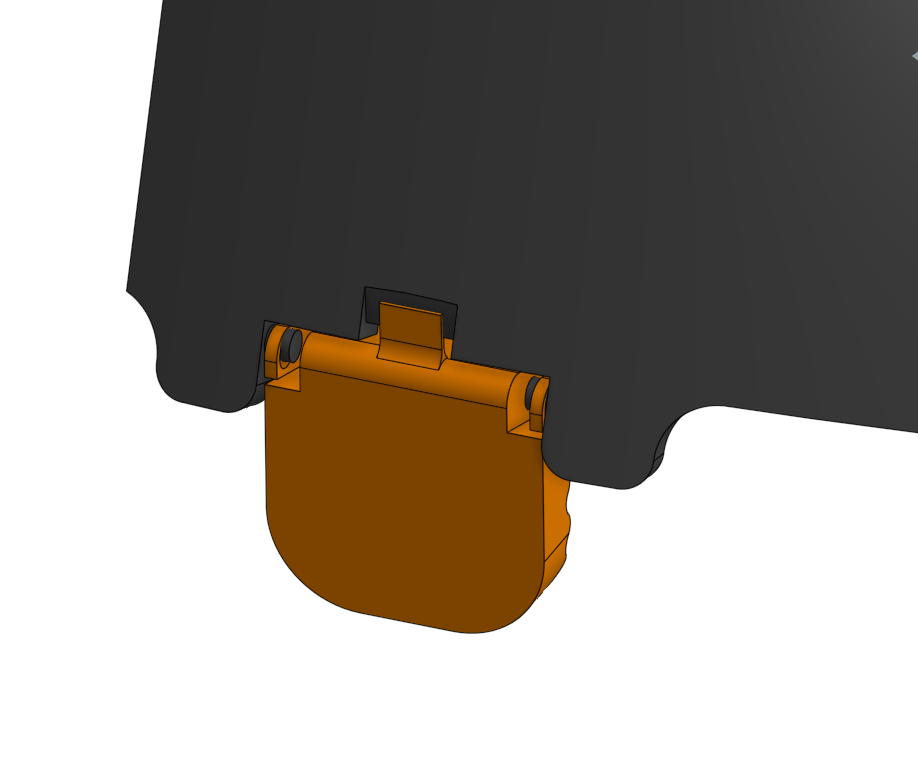
\includegraphics[width=0.4\textwidth]{graphics/flexible_nub1.png}
    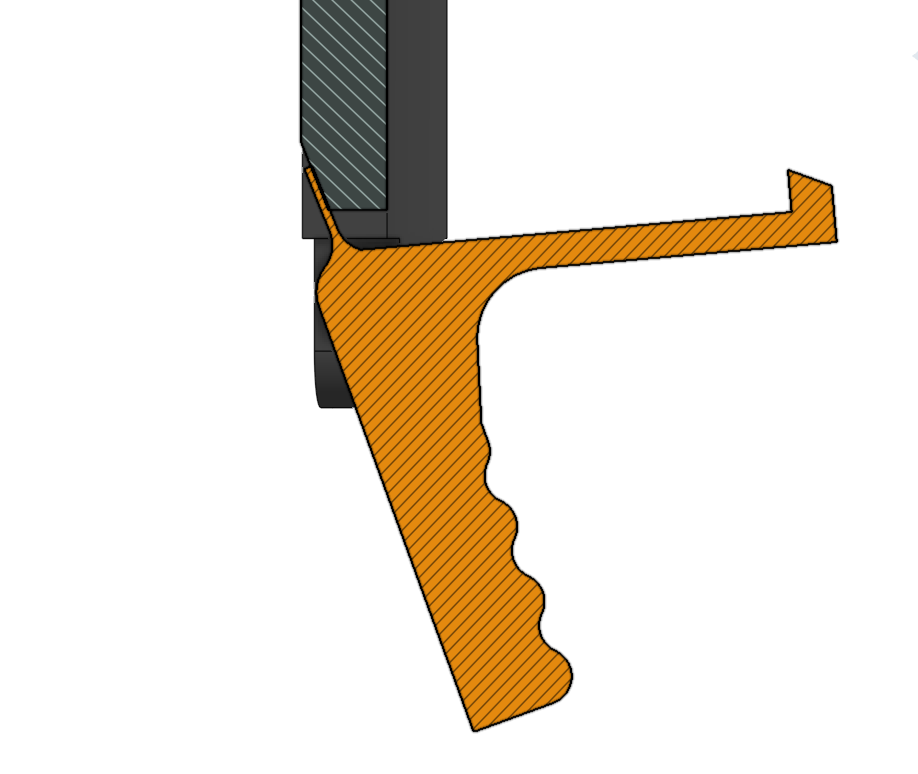
\includegraphics[width=0.4\textwidth]{graphics/flexible_nub2.png}\\
    CAD models of the flexible nub design. A flexible nub on the clamp would rest against a notch in the shell which would prevent it from rotating keeping the latch in place.
\end{figure}

The issues with this design was that it significantly overestimated the strength and flexibility of the parts. When you are making parts in CAD it is easy to forget how small the parts that are being designed actually are. A design like this isn't possible because such a thin nub will shear off under the loads it is supposed support.

\subsection{Vertical Leaf Spring}

The next idea was to have a much larger leaf spring by making the shell the flexible segment and the nub the rigid one. A benefit to orienting the leaf vertically is that this requires no support material. This idea didn't work out because the flexural strength of FDM printed parts is much worse between layers and designs like this were too brittle.

\begin{figure}[h!]
    \centering
    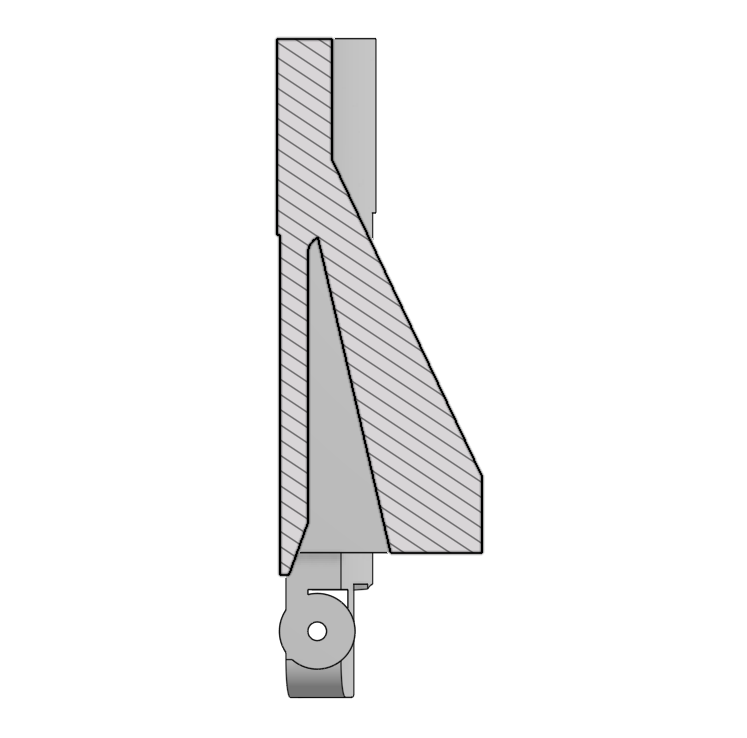
\includegraphics[width=0.4\textwidth]{graphics/vertical_leaf1.png}
    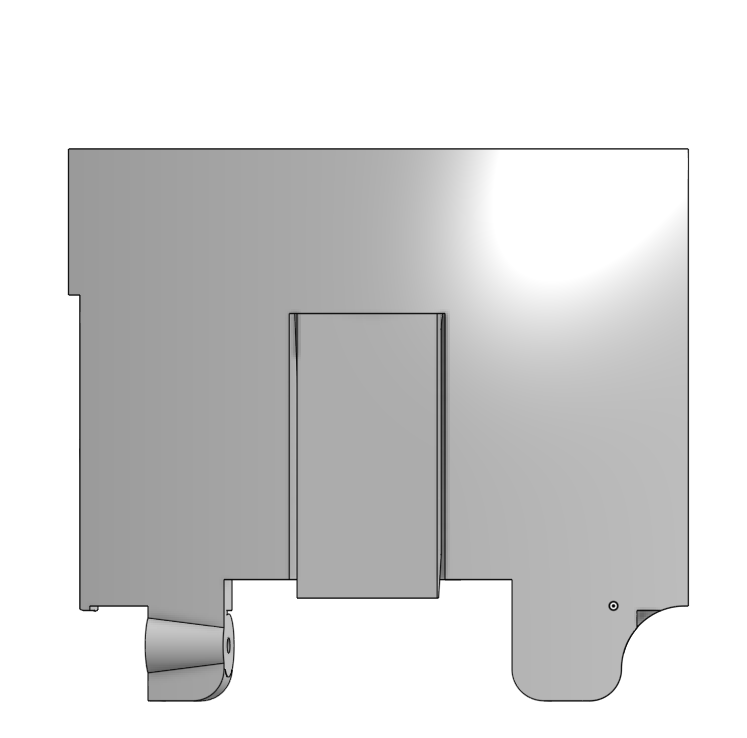
\includegraphics[width=0.4\textwidth]{graphics/vertical_leaf2.png}\\
    CAD model of a shell with a vertical leaf spring which could flex backwards into the shell.
\end{figure}

%\section{Future improvements}

\end{document}